
In Sect.~\ref{se:toi_proc}, we have introduced the TOI properties of the
instrument and our reference data reduction scheme. We here go up to the final
maps while considering the time spent observing to derive the sensitivity of the
instrument, \aka\ the \emph{Noise Equivalent Flux Density}, (NEFD).\\

The MoU defines the NEFD:  \emph{The Noise Equivalent Flux Density (NEFD)
  is the $1\,\sigma$ sensitivity in one second of effective on-source telescope
  integration time after the absolute calibration has been performed (i.e. after
  beam efficiency and opacity corrections). It is appropriate for 2 mm of
  precipitable water vapor (pwv) content in the atmosphere and 60 degrees
  elevation source. It refers to the inverse variance of the noise on the flux
  measurement of a point-source, averaged over the valid receiver pixels}.\\

IRAM has its own time estimator for astronomers that will compute the ``effective NEFD'',
provided we give the ``detector NEFD'' and a fraction of valid KIDs $\eta$. To
derive the detector NEFD, we must clearly define the ``detector time of
integration'' and relate it to the ``time of observation'' which is the time
actually spent by an astronomer at the observing desk. Going from the intuitive
understanding of the time of integration to its actual value is not as trivial
as it seems because of the dependence on the scanning strategy and the
distribution of valid KIDs across the FOV.

\section{Estimating the time of integration}

\subsection{Time of integration from the density of samples}

Let's take a map of resolution $r$ (arcsec) and consider the map pixel that is
centered on the position where we estimate the flux uncertainty
$\sigma_\phi$. The number of hits in this pixel $N_{\rm{h}}(r)$ allows us to define a
time of integration on this pixel via the sampling frequency $\nu$

\begin{equation}
t_{pix} = N_h(r)/\nu
\end{equation}

To estimate how much wall clock time was necessary to the entire matrix to
produce this density of samples, we need to account for how many KIDs, on
average, contribute to $N_{\rm{h}}(r)$ at the same time, that is to say the average
number of KIDs per map pixel. Indeed, if the pixel is large enough to contain
$n$ KIDs at each time, the number of samples in this pixel will be $n$ times
larger for the same time of observation. The same is true if we combine A1 and
A3 for instance. We therefore note $S$ the surface of the FOV, $g$ the distance
between adjacent KIDs and note that $S = N_{\rm{pix}} \times r^2 = N_{\rm{KID}} \times
g^2$. The number of KIDs per pixel of $r$\,arcsec resolution is thus $r^2/g^2$,
so the actual observation time reads

\begin{equation}
t_{\rm{det}} = t_{\rm{pix}}\frac{g^2}{r^2} = \frac{N_{\rm{h}}(r)}{\nu}\frac{g^2}{r^2}
\end{equation}

For the combination of arrays 1 and 3, the number of KIDs per pixel is the sum
of the two contributions that impact the number of KIDs per pixel:

\begin{equation}
t_{\rm{det}}^{1mm} = \frac{1}{2}\frac{N^{1\rm{mm}}_{\rm{h}}(r)}{\nu}\frac{g^2}{r^2}
\end{equation}

So finally, if $\sigma_\phi$ is the uncertainty on the flux estimate, the detector NEFD reads

\begin{equation}
NEFD_{\rm{det}} = \sigma_\phi\sqrt{t_{\rm{det}}}
\label{eq:nefd_t_int}
\end{equation}

To relate it to the effective ``observer'' NEFD, we must account for the
fraction of valid pixels actually used to derive the map. Indeed, the
integration time per pixel goes like $\eta$ for the same observation, thus:

\begin{equation}
NEFD_{\rm{det}}^{\rm{eff}} = \sigma_\phi\sqrt{t_{\rm{det}}/\eta}
\end{equation}

which in turn translates into a time requirement to reach the same level of integration:

\begin{equation}
t_{\rm{det}}^{\rm{req}} = \left(\frac{NEFD_{\rm{det}}}{\sigma_\phi}\right)^2\frac{1}{\eta}
\label{eq:t_astro}
\end{equation}

\subsection{Time of integration from the matrix footprint}

One can also think at the ``time spent on the source'', for a full matrix
(ie. all valid KIDs), as the time when the source is inside the circular
footprint of the matrix. During a scan, it's easy to count how much time the
source is at a distance from the FOV center that is smaller than the FOV
radius. This time, $t_{geom}$ is a direct estimate of the time ``at the desk'',
so it enters the definition of effective NEFD, not the detector NEFD, hence:

\begin{equation}
NEFD^{\rm{eff}}_{\rm{geom}} = \sigma_\phi \sqrt{t_{\rm{geom}}}
\end{equation}

Fig.~\ref{fig:time_comparison} compares $\eta t_{\rm{geom}}$ to $t_{\rm{det}}$ and shows
the good agreement between the two. Because the definition of $t_{\rm{det}}$ is more
straightforward in terms of measurement from the map and design parameters and
does not require an approximate determination of the FOV radius, it is 
\emph{our reference time estimator}.

\todo{MARCO'S COMMENT: $t_{det}$ is always lower than $\eta*t_{geom}$
(see Fig.8.1); a possible origin of that should be that $t_{det}$ is
underestimated.
In fact, the number of KIDs per pixel of $r$ arcsec resolution is
estimated as $r^2/g^2$ but, due to pixel interspaces, this number is
overstimated and so $t_{det}$ underestimated. LP: oui, ou alors
certains samples ont ete flaggues et ne sont pas comptes dasn la carte
de hits (Nico, tu penses qu'il faut ajouter un commentaire ?)}

\begin{figure}[!thbp]
\begin{center}
\includegraphics[clip, angle=0, scale =0.8]{Figures/time_of_integration_0.eps}
\caption[Time of integration]{Comparison between two estimators of the time of
  integration on \hls\ during Run~9 for FOV diameter of 6.2~arcmin. The
  difference goes from 2\% to 5\%, hence translating into a NEFD relative difference of 1
to 2.5\%.}
\label{fig:time_comparison}
\end{center}
\end{figure}

%% \subsubsection{Time of integration from the flux estimator}
%% 
%% The estimation of the flux of a point source, and its associated uncertainty is
%% done by fitting the amplitude of a gaussian profile of fixed FWHM. In the case
%% of white noise, the flux estimator reads
%% 
%% \begin{equation}
%% \hat{\phi} = \frac{1}{\sum_p g_p^2}\sum_p g_p m_p\,,
%% \label{eq:phi_def}
%% \end{equation}
%% 
%% and its variance is
%% 
%% \begin{equation}
%% \sigma_\phi^2 = \left(\frac{1}{\sum_p g_p^2}\right)^2\sum_p g_p^2\sigma_p^2\,.
%% \label{eq:sigma_phi_def}
%% \end{equation}
%% 
%% In the case of white noise and considering the equivalent of the
%% uniform full matrix of the NEFD definition: $\sigma_p = \sigma_1/\sqrt{N_p}$,
%% where $\sigma_1$ is the standard deviation of 1 sample and $N_p$ is the number of
%% hits in pixel $p$. Accounting for the sampling frequency, it reads
%% 
%% \begin{eqnarray}
%% \sigma_\phi^2 &=& \frac{\sigma_1}{\nu}\left(\frac{1}{\sum_p g_p^2}\right)^2\sum_p \frac{g_p^2}{t_p}\,, \nonumber\\
%% &=&\frac{\sigma_1}{\nu}\frac{1}{t_{beam}}\,
%% \label{eq:sigma_phi_def_2}
%% \end{eqnarray}
%% 
%% where $t_{beam}$ is homogeneous to a time and is such that $\sigma_\phi$ goes
%% like $1/\sqrt{t_{beam}}$.


\section{NEFD estimation methods}
\label{se:nefd_estimation_methods}

With the uncertainty on flux measurements as described in Sect.~\ref{se:photometry} and
now an estimator of the time of integration, we have everything in hand to derive
the NEFD. We have devised several ways to estimate it at the same time as
checking the good behaviour of the instrument. Two methods are based on deep
integrations on a source, one is based on the joint analysis of multiple scans
without combining them:

\begin{enumerate}
\item {\bf Deep Integration method 1}: the error on the flux of a point source for an
  integration time $t$ is $\sigma_\phi(t) = NEFD/\sqrt{t}$. Co-adding several scans of
  the same source and fitting $\sigma_\phi$ as a function of the
  inverse of the square root of the
  time of integration must therefore give a straight line whose
  amplitude is the NEFD if correctly corrected for the different elevation and
  opacity conditions of observations.
\item {\bf Deep Integration method 2}: by summing a large and even number of scans
  with alternate positive and negative weights, we cancel the signal while
  keeping the noise properties. This final ``Jackknife'' map can then be analyzed
  to provide estimates of flux uncertainties for a the effective time of
  integration, hence giving an alternative estimation of the NEFD.
\item {\bf Scatter method}: analyzing each scan in terms of sensitivity and
  time of integration, we have a NEFD per scan that varies with opacity and
  elevation. Fitting the distribution of measures against $exp(\tau/sin\delta)$
  provides the zenith NEFD.
\end{enumerate}

In this section, we use first two data sets from Runs 9 and 12 and
\new{then all the scans of sub-Jy sources acquired during Runs 9, 12 and
14.} 

For Run~9, we use observation scans towards \hls\, which is a
moderately faint source \cite{hls_combes}, expected to be
74.5\,mJy at 1mm and 15.7\,mJy at 2mm (M.~Bethermin, private
communication). This source was chosen for its flux and its availability during
Run9 for long integration. It has been observed for about 9\,h in total over
three nights. The scans were 8x5~arcmin$^2$, alternatively oriented in (ra,dec),
(dec,ra), (az,el), (el,az). \samu{The rational for this scan strategy
is twofold. First, it makes the filtering due to the data
reduction more isotropic to avoid the presence of spurious priviledged directions in
the map. Second, it provides the required redundancy in the mapping
to allow the use of dedicated denoising algorithms (a.k.a. destriping codes).}

For Run~12, G2 has become the nickname of an empty target close to sources known
to IRAM but not to the commissioning team in order to check our source
detection capabilities blindly.

The data were processed according to Sect.~\ref{se:pipeline_overview}.

\subsection{Deep integration method 1: $\sigma = NEFD/\sqrt{t}$}
\label{se:nefd_m1}

%%  and the
%% scans have 
%% \hls. The scans have been combined with standard inverse noise weighting. The
%% noise in each map pixel is derived from the rms of the background corrected by
%% the square root of the number of observations per pixel (N1). If the noise was
%% perfectly gaussian, the distribution of the map signal over this noise estimate
%% (far from the source) would be a normalized gaussian. In practice, this leads to
%% gaussians that 1.6 and 1.5 larger. We therefore increase our noise estimate (N1)
%% by these factors to derive our final estimates. Should the extra sources that
%% pop up in the field contribute to this estimate, they would only make our
%% estimate more conservative.

We co-add the scans one by one and each time perform a photometric analysis on
the map according to Sect.~\ref{se:photometry}. The uncertainty on the flux at
the center of the field (on source in the case of \hls, off source in the case
of G2) is plotted and fitted against $\sqrt{t_{\rm{det}}}$. It should go like a
straight line if scans were all taken in the exact same conditions and stacked
with equal weights. In practice, the weights are sensitive to the conditions of
observation, namely the elevation and opacities (see Fig.~\ref{fig:nefd_plots})
and this weight variation must be accounted for. The uncertainty on
the central flux reads

\begin{equation}
\sigma = NEFD_{\rm{det}}\times e^{\tau/\sin\delta}\,t^{-1/2}
\label{eq:sigma_nefd}
\end{equation}

Because scans are coadded with inverse variance weighting, the combined flux is

\begin{equation}
\phi = \frac{1}{\sum_n 1/\sigma_n^2}\sum_n\frac{\phi_n}{\sigma_n^2}
\end{equation}

whose variance is

\begin{equation}
\sigma^2 = \frac{1}{\sum_n 1/\sigma_n^2}
\end{equation}

which, according to Eq.~(\ref{eq:sigma_nefd}) becomes

\begin{equation}
\sigma^2 = \frac{NEFD_0^2}{\sum_{n}t_n e^{-2\tau_n/\sin\delta_n}}\,.
\label{eq:sigma_tau_w8}
\end{equation}

If the opacity and the elevation were the same for all scans, we recover the
integration like $\sqrt{t}$. In general, if the observing conditions vary, we
must fit the integrated sensitivity vs the effective time $\sum_{n}t_n
e^{-2\tau_n/\sin\delta_n}$ in order to recover an unbiased estimate of
$NEFD_0$. The method was applied to \hls\ and G2, results are summarized on
Fig.~\ref{fig:nefd_plots} and in Tab.~\ref{tab:nefd_summary}.

\begin{figure}[!thbp]
\begin{center}
\includegraphics[clip, angle=0, scale =0.42]{Figures/hls_nefd_vst.eps}
\includegraphics[clip, angle=0, scale =0.42]{Figures/g2_nefd_vst.eps}
\includegraphics[clip, angle=0, scale =0.4]{Figures/hls_opacity_and_elev.eps}
\includegraphics[clip, angle=0, scale =0.4]{Figures/g2_opacity_and_elev.eps}
\caption[NEFD vs time]{\emph{Top row:} 1\,$\sigma$ sensitivity on the
  measure of the flux of a point source vs the time of integration on this
  source in two cases. The sensitivity goes like $t^{-1/2}$ as
  expected. \emph{Bottom row:} Opacities and elevations of the scans used in
  this analysis. \new{The average opacities at $1$ and $2\,\rm{mm}$ are
  given in the legend.}}
\label{fig:nefd_plots}
\end{center}
\end{figure}

\subsection{Deep integration method 2: Jackknife}

With enough scans of the same source, it is possible to alternate addition and
subtraction of the scans and therefore cancel the contribution of the signal to
the final combination, while preserving the noise properties. This method is
often referred to as ``Jackknife'' and is a powerful test for residual
systematics. The Jaccknife maps of \hls\ and G2 are presented on
Fig.~\ref{fig:jk_maps}. Photometry at their center provides estimates of the
\samu{top-of-atmosphere} NEFD that are reported in Tab.~\ref{tab:nefd_summary}.

\begin{figure}[!thbp]
\begin{center}
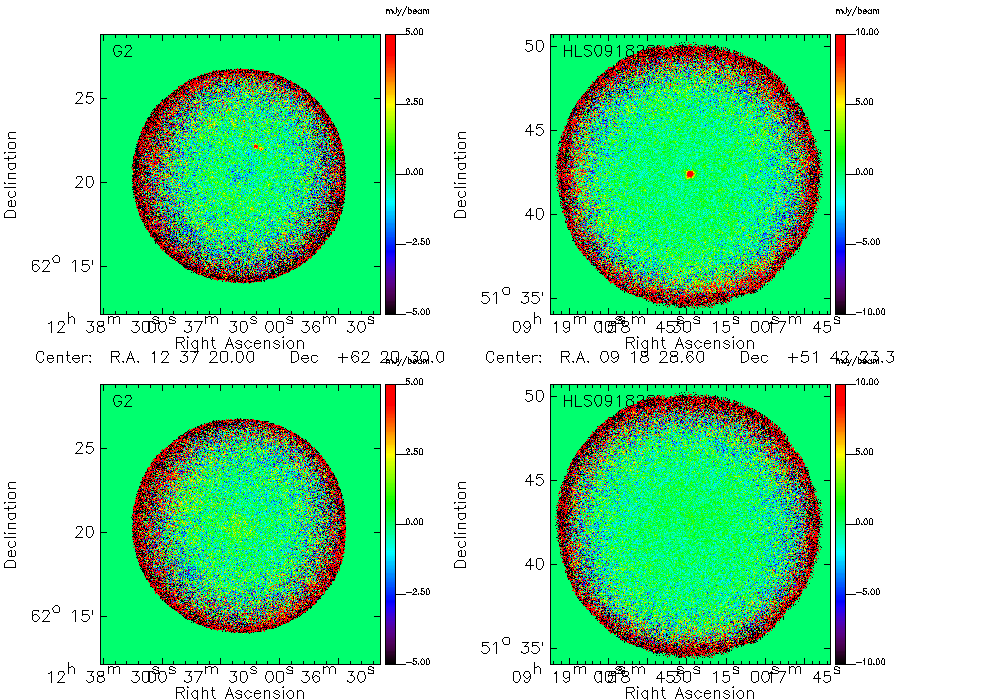
\includegraphics[clip, angle=0, scale=0.5]{Figures/nefd_jackknife.png}
\caption[Jackknife maps of G2 and \hls]{\emph{Top row:} Maps of \hls\ and G2 at
  $1\,\rm{mm}$. \emph{Bottom row:} \emph{Jackknife} maps at
  $1\,\rm{mm}$. After the sum of scans with alternate positive and negative
  weights, signal residuals are negligible while noise properties are preserved.}
\label{fig:jk_maps}
\end{center}
\end{figure}


\subsection{NEFD per scan vs $e^{\tau/sin\delta}$: Scatter}
\label{se:nefd_scatter}

Performing photometry on each individual scan on G2 or \hls, we can estimate the
sensitivity on the central flux and measure the time of integration, hence
derive the NEFD for this scan. This determination is intrinsically noisier than
the two previous maps because of the variance associated to each scan. However,
taken all together, the scans provide another estimate of the instrument
NEFD. Results are presented on Fig.~\ref{fig:nefd_scatter} and the derived
\samu{top-of-atmosphere} NEFD are given in Tab.~\ref{tab:nefd_summary}.

\begin{figure}[!thbp]
\begin{center}
\includegraphics[clip, angle=0, scale =0.42]{Figures/hls_NEFD_vs_TauElev_all.eps}
\includegraphics[clip, angle=0, scale =0.42]{Figures/g2_NEFD_vs_TauElev_all.eps}
\caption[NEFD per scan]{1\,$\sigma$ sensitivity on the central flux for each
  observation of G2 and \hls. The solid black line is the theoretical
  fit of $\rm{NEFD} = \rm{NEFD}_0$ $e^{(\tau/\sin\delta)}$
  %$\sigma = \sigma_{ref}e^{\tau/\sin\delta}$
  and gives the NEFD when extrapolated to $\tau/\sin\delta = 0$.}
\label{fig:nefd_scatter}
\end{center}
\end{figure}

While the two first methods require long integration on the same source, this
\emph{scatter} method can be used on all scans. In practice, noise
characterization may be biased by residuals of a strong source and the
instrument far side lobes (Fig.~\ref{fig:nefdvsbackground}). We therefore
restrict to sources with a flux below
1\,Jy. Fig.~\ref{fig:nefdvsbackground_below_1Jy} further shows the comparison
between runs N2R9, N2R12 and N2R14 and their consistency.

\begin{figure}[!thbp]
\begin{center}
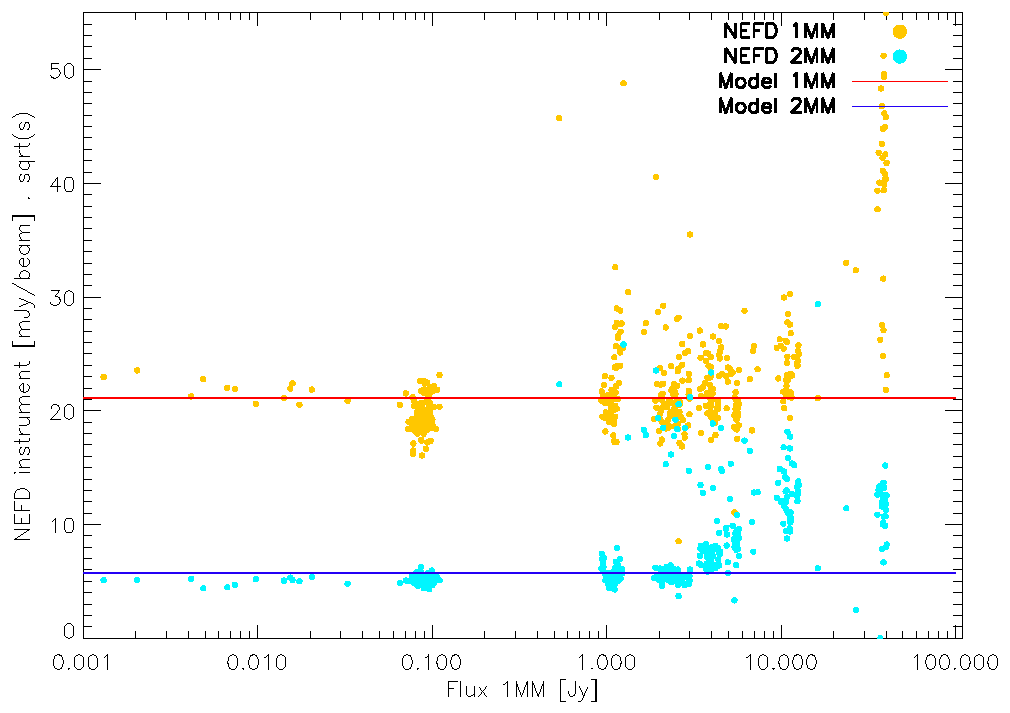
\includegraphics[clip=true,width=0.47\textwidth]{Figures/NEFDIndScans/nefd_flux1mm_run22.pdf}
\caption[Measured NEFD versus source flux for N2R9 at 1 and 2 mm]{Measured NEFD
  versus source flux for N2R9 at 1 and 2 mm using the \emph{scatter} method}
\label{fig:nefdvsbackground}
\end{center}
\end{figure}

\begin{figure}[!thbp]
\begin{center}
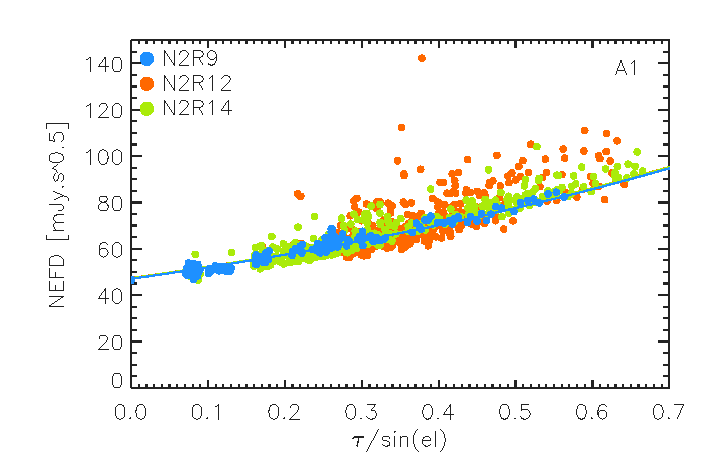
\includegraphics[clip=true,width=0.47\textwidth]{Figures/NEFD/plot_nefd_vs_obstau_corrected_skydip_vfinal_a1.pdf}
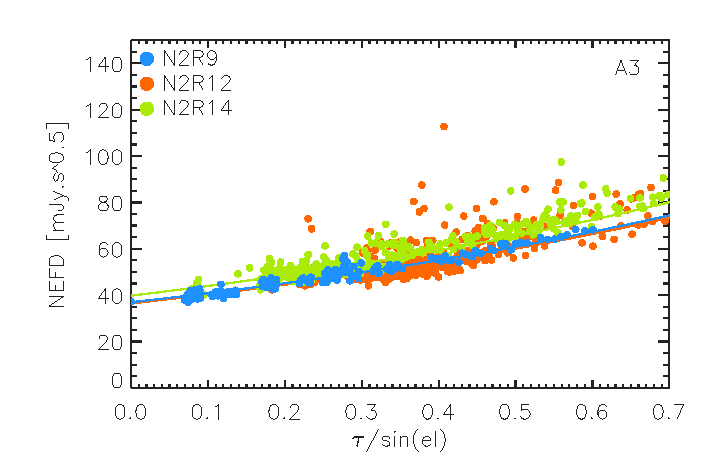
\includegraphics[clip=true,width=0.47\textwidth]{Figures/NEFD/plot_nefd_vs_obstau_corrected_skydip_vfinal_a3.pdf}
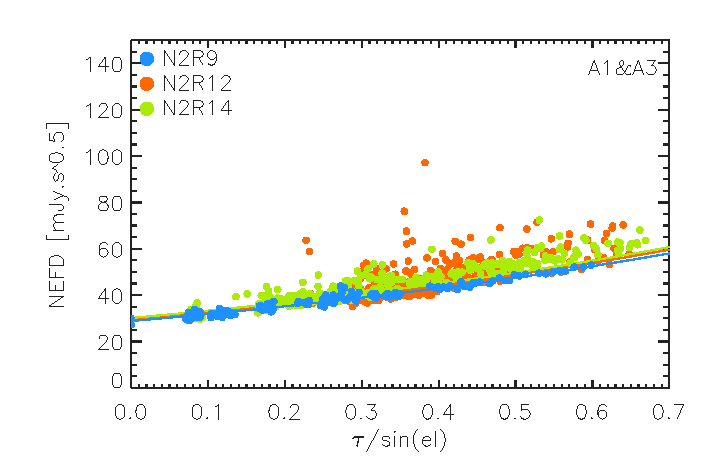
\includegraphics[clip=true,width=0.47\textwidth]{Figures/NEFD/plot_nefd_vs_obstau_corrected_skydip_vfinal_1mm.pdf}
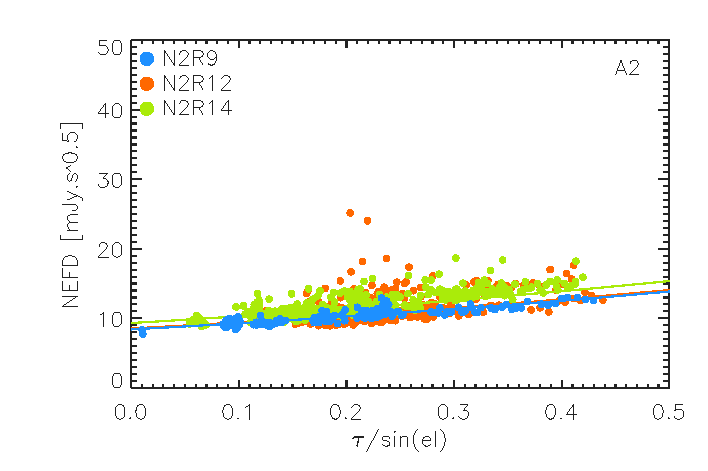
\includegraphics[clip=true,width=0.47\textwidth]{Figures/NEFD/plot_nefd_vs_obstau_corrected_skydip_vfinal_a2.pdf}
\caption[Measured NEFD versus observed opacity]{Measured NEFD as a function of
  line-of-sight opacity ($\tau/sin(\delta)$) for array 1 (upper left), array 3 (upper right), the
  $1~\rm{mm}$ (lower left) and $2~\rm{mm}$ (lower right)
  channels. Data points
  are NEFD estimates in mJy.s$^{1/2}$ for N2R9 (blue), N2R12 (orange)
  and N2R14 (chartreuse). We also show in the plots the expected NEFD evolution
  with the line-of-sight opacity as solid curves \new{using the median
  zenith opacity derived from all the scans acquired during a campaign.}}
\label{fig:nefdvsbackground_below_1Jy}
\end{center}
\end{figure}
 

\begin{table}[!thbp]
\begin{center}
\begin{tabular}{|l|l|c|c|c|c|c|c|}
  \hline
  \multicolumn{2}{|c|}{}  & \hls   & G2    &    \multicolumn{4}{|c|}{<1\,Jy}  \\\cline{5-8}
  \multicolumn{2}{|c|}{}  &        &       &  N2R9 & N2R12 & N2R14 & Combined \\
\hline
{\it Scatter} & A1        & 45.7   & 47.2 &  47.0 &  47.3 &  47.3 &  47.2 \\
              & A3        & 36.3   & 37.3 &  36.9 &  36.4 &  39.8 &  37.9 \\
              & A1\&A3    & 28.5   & 30.3 &  28.8 &  30.2 &  30.9 &  30.1 \\
              & A2        &  8.2   &  8.9 &  8.4  &   8.5 &   9.3 &   8.8 \\
\hline
{\it Jackknife} & A1      & 48.1   & 52.1 & \multicolumn{4}{|c|}{}  \\
                & A3      & 37.5   & 38.8 & \multicolumn{4}{|c|}{}  \\
                & A1\&A3  & 29.0   & 32.2 & \multicolumn{4}{|c|}{}  \\
                & A2      &  8.9   & 10.9 & \multicolumn{4}{|c|}{}  \\
\hline
$t^{-1/2}$  & A1          & 46.6   & 44.0 & \multicolumn{4}{|c|}{} \\
            & A3          & 38.4   & 34.7 & \multicolumn{4}{|c|}{} \\
            & A1\&A3      & 30.4   & 29.6 & \multicolumn{4}{|c|}{} \\
            & A2          &  8.5   &  7.8 &\multicolumn{4}{|c|}{}  \\
\hline
\end{tabular}
\caption[Comparison of the NEFD estimates using three methods]{NEFD's in mJy.s$^{1/2}$ for the three methods described in the text
  and obtained on G2, \hls, and all sub-Jy sources of runs N2R9,
  N2R12, N2R14. The results given in the last column are based on more
  than a thousand scans, which distribute as 202, 481 and 430 scans of
  N2R9, N2R12 and N2R14 respectively.}
\label{tab:nefd_summary}
\end{center}
\end{table}


Combining the data set of N2R9, N2R12 and N2R14 campaigns,
more than one thousand observations scans of sub-Jy sources meet the
baseline selection criteria (see Sect.~\ref{se:data_selection}),
providing us with robust NEFD estimates that are representative of
average NIKA2 performance, which are gathered in
Tab.~\ref{tab:nefd_astro}.
The \samu{top-of-atmosphere} NEFD and RMS uncertainties are evaluated as the median and
the scatter of the individual NEFD corrected with
$\exp[\tau/sin(\delta)]$. These values are then extrapolated at the
reference IRAM observing conditions, which consists of $2~\rm{mm}$
of precipitable water vapor (pwv) in the atmosphere and $60$ degrees
elevation.


%% LP
To further estimate the mapping capabilities, we also evaluate the
mapping speed $M_{\rm{s}}$, which is defined as the sky area that is covered in one
hour of observation to a noise level of $1\,\rm{mJy}$, using
\begin{equation}
M_{\rm{s}} = \frac{\pi}{4} d_{\rm{FoV}}^2 \, \frac{\eta}{\rm{NEFD}^2},
\end{equation}
where $d_{\rm{FoV}} = 6.5'$ is the FoV diameter and $\eta$ the
fraction of valid KIDs, as given in Tab.~\ref{tab:number_of_kids} in
Sect.~\ref{se:fov_geometry}.
The mapping speed that is extrapolated at zero opacity, and the astronomer
mapping speed that is extrapolated at the reference IRAM observing conditions are
given in Tab.~\ref{tab:nefd_astro}.   
%eta  = [0.84, 0.84, 0.84, 0.90]
%nefd0 = [47.2, 37.9, 30.1, 8.8]
%ms0   = !dpi/4.0d0*6.5d0^2*eta/nefd0^2*60.0d0^2 ;; arcmin^2/h/mJy^2
%print, ms0
%nefda = [56.6, 45.6, 36.1, 9.8]
%msa   = !dpi/4.0d0*6.5d0^2*eta/nefda^2*60.0d0^2 ;; arcmin^2/h/mJy^2
%print, msa

\begin{table}[!thbp]
\begin{center}
\begin{tabular}{|l|c|c|c|c|}
  \hline
 <1 Jy               & A1      &   A3    &   A1\&A3 &    A2    \\  
\hline\hline
NEFD\small{(0mm, 90deg)}             & 47.2    & 37.9    &    30.1  &    8.8   \\
RMS NEFD\small{(0mm, 90deg)}         &  3.9    &  3.5    &     2.9  &    1.1   \\
M$_{\rm{s}}$\small{(0mm, 90deg)}      & 45      &  70     &    111   &   1388   \\
\hline
NEFD\small{(2mm, 60deg)}         & 56.6    & 45.6    &    36.1  &    9.8   \\
RMS NEFD\small{(2mm, 60deg)}     &  4.7    & 4.2     &     3.5  &    1.2   \\
M$_{\rm{s}}$\small{(2mm, 60deg)}  &  31    & 48       &    77   &   1119   \\
\hline
\hline
\end{tabular}
\caption[NEFD estimates on all sub-Jy sources]{Median NEFD and rms
uncertainties in $\rm{mJy}\cdot \rm{s}^{1/2}$, as well as the derived mapping
speed in $\rm{arcmin}^2\cdot\rm{mJy}^{-2}\cdot\rm{h}^{-1}$, evaluated
in using the scatter method on all sub-Jy sources of runs N2R9, N2R12
and N2R14, given at pwv=0 and 90 degrees elevation (first three rows) and extrapolated at the
reference IRAM observing conditions (last three rows), which are defined
as $2\,\rm{mm}$ pwv and 60 degrees elevation.}
\label{tab:nefd_astro}
\end{center}
\end{table}


%% Baseline astromoner and instrument NEFD results are gathered in
%% Table.~\ref{tab:baseline_nefd_pipeline}.
%% 
%% \begin{table}
%% \begin{center}
%% \begin{tabular}{|c|c|rrrr|}
%% \hline
%% NEFD type & Arrays & N2R9 & N2R12 & N2R14 & Combined  \\
%% \hline\hline
%% Astronomer  & A1       &  64.8 & 63.6 &  58.7 &  62.7 \\
%%             & A3       &  48.3 & 47.3 &  47.7 &  47.7 \\ 
%%             & A1 \& A3 &  38.0 & 38.9 &  37.9 &  38.3 \\
%%             & A2       &   9.4 &  9.4 &   9.8 &   9.5  \\
%% \hline
%% Instrument  & A1       &   54.0 & 53.1 &  49.0 & 52.3  \\
%%             & A3       &   40.1 & 39.3 &  39.6 & 39.6  \\ 
%%             & A1 \& A3 &   31.6 & 32.3 &  31.5 & 31.9  \\
%%             & A2       &    8.5 &  8.5 &  8.9  &  8.6  \\
%% \hline\hline
%% \end{tabular}
%% \label{tab:baseline_nefd_pipeline}
%% \caption[NEFD using method 3]{Astromoner (average IRAM observing conditions) and Instrument (zero opacity) NEFD estimates in mJ.s$^{0.5}$ for N2R9, N2R12 and N2R14 campaigns and for the union of the observations acquired during the three campaigns, that are more than a thousand scans. }
%% \end{center}
%% \end{table}



